\chapter{双频激光干涉仪的环境误差补偿实验系统}
\section{双频激光干涉仪测量系统光路设计与分析}
\section{基于PT100的八通道温度测量系统}
本文工作所采用的温度传感器为基于PT100电阻的多通道温度测量系统,最多支持8个通道的同时测量,供电电压为\(+12 \sim +24VDC\),能够支持\(22^{\circ}C \pm 5^{\circ}C\)范围内的温度测量,测量精度\(\leq \pm 0.04^{\circ}C\)。
\subsection{上位机系统}
基于PT100电阻的多通道温度测量系统上位机采用美国国家仪器(NI)公司研制开发的LabVIE程序开发环境开发,并且需要NI LabVIEW Runtime和NI-VISA模组。该上位机软件能够实现数据的测量、显示、存储并且自带标定数据分析功能,上位机软件流程图以及部分关键代码如图所示。

程序的面向用户界面如图\ref{fig:温度测量上位机前面板}所示,
\begin{figure}[htb]
    \centering
    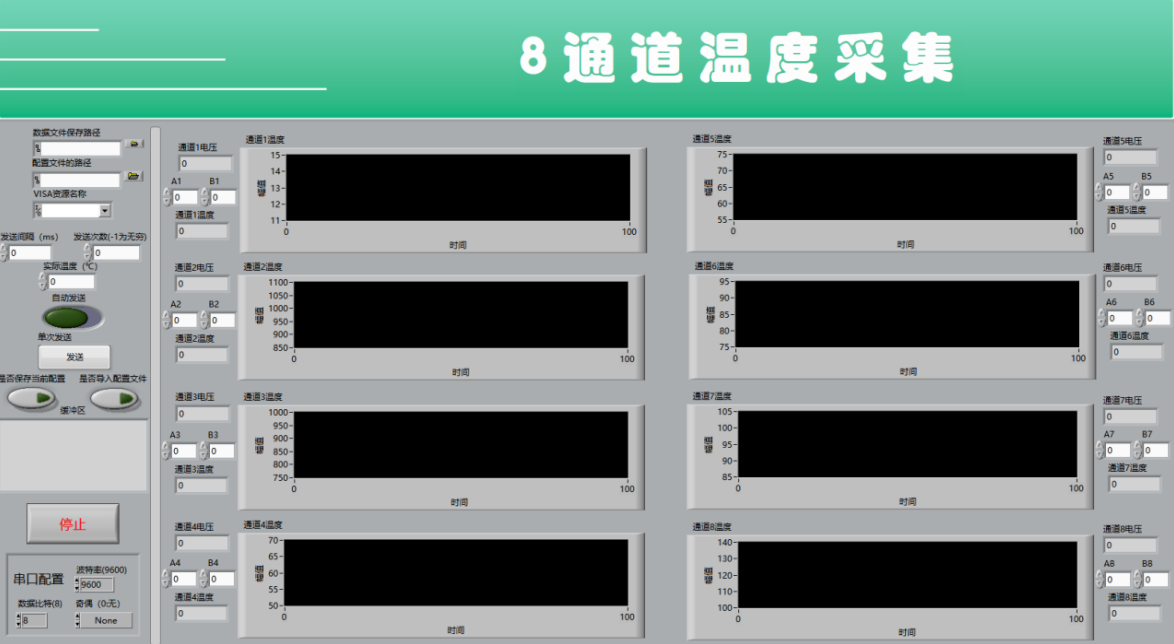
\includegraphics[width=14cm]{fig/3-fig/温度采集上位机前面板.jpg}
    \caption{温度测量上位机前面板}
    \label{fig:温度测量上位机前面板}
\end{figure}

图\ref{fig:温度测量上位机前面板}右边可见8个通道当前的标定系数,以及温度的实时测量值,而过去一段时间内的温度测量值的变化趋势则会以曲线的形式显示,用户界面的左列则为用户控制区,可进行以下参数的设定:
\begin{enumerate}
    \item 数据文件保存路径:选择测量数据保存的文件夹,程序会自动在该文件夹产生csv文件,文件的命名格式为年月日,如20210129。
    \item 配置文件的路径:选择配置文件路径,上位机软件会根据该配置文件里的系数计算温度值,配置文件通常由程序自带标定拟合功能产生。
    \item 自动发送:自动采集模式与手动采集模式的选择开关,若为自动采集模式,则根据“发送间隔”和“发送次数”两个参数,每隔一段时间进行一次采集,达到采集次数之后程序停止;若为手动采集模式则每次单机“发送”按钮后进行一次采集。
    \item 发送间隔:自动发送模式下,每次发送采集命令之间的时间间隔。
    \item 发送次数:自动发送模式下,发送采集命令的总次数(即采集次数),-1为无穷次。
    \item 实际温度:用于记录当前的实际温度,会在产生的csv文件中有记录,该项主要用于系统标定时。
    \item 串口配置:设置串口的波特率、数据比特位宽以及奇偶校验位。
  \end{enumerate}

  \subsection{标定过程及结果}
  基于PT100电阻的多通道温度测量系统标定过程如图\ref{fig:标定示意图}所示,在中空的热承中灌导热系数较好的油,并在热承下放置半导体制冷片,半导体制冷片下方放置散热片,两者接触面均匀涂抹导热硅脂,其余位置用黑色保温棉包裹,将待标定的PT100温度传感器捆绑在一起,减少温度不均性带来的误差。使用TCM-X107数字温控模块控制半导体制冷片,并在\(16^{\circ}C \sim 26^{\circ}C\)范围内取定几个温度点作为标定点,采用高精度温度传感器T520进行标定,每个标定待温度稳定之后,以\(0.5Hz\)的采样频率,采集一百个数据,去除最大值和最小值之后,以这98个点的平均值作为待标定数据。
  \begin{figure}[htb]
    \centering
    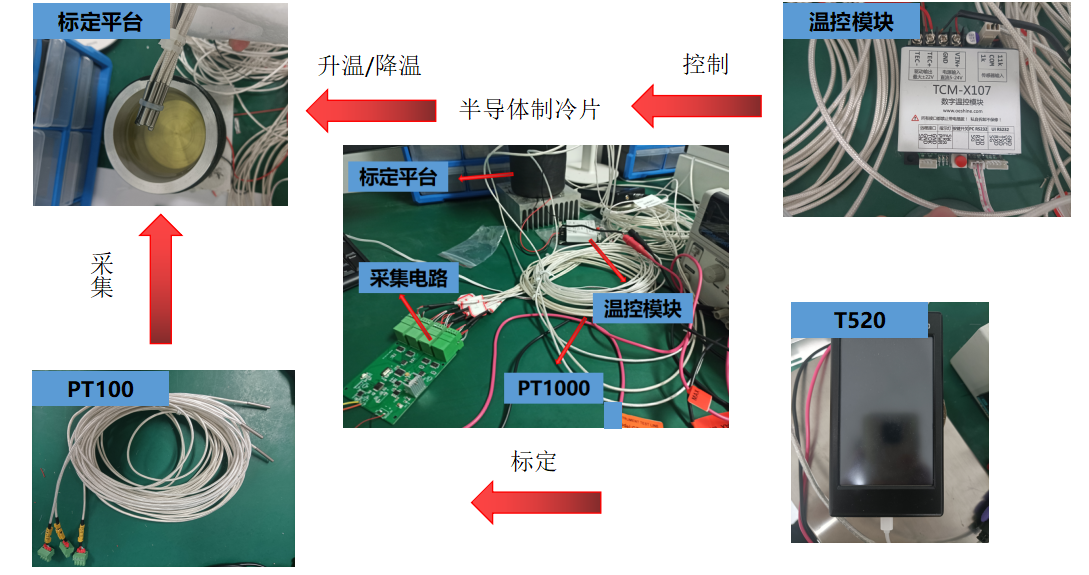
\includegraphics[width=12cm]{fig/3-fig/温度测量系统标定示意图.jpg}
    \caption{标定示意图}
    \label{fig:标定示意图}
\end{figure}

标定程序界面如图\ref{fig:标定程序用户界面}所示,红色的点为8个通道采集到的离散的温度数据,蓝色曲线为标定程序输出的拟合曲线,程序会自动根据标定结果生成.ini配置文件,供测量系统上位机使用。
\begin{figure}[htb]
    \centering
    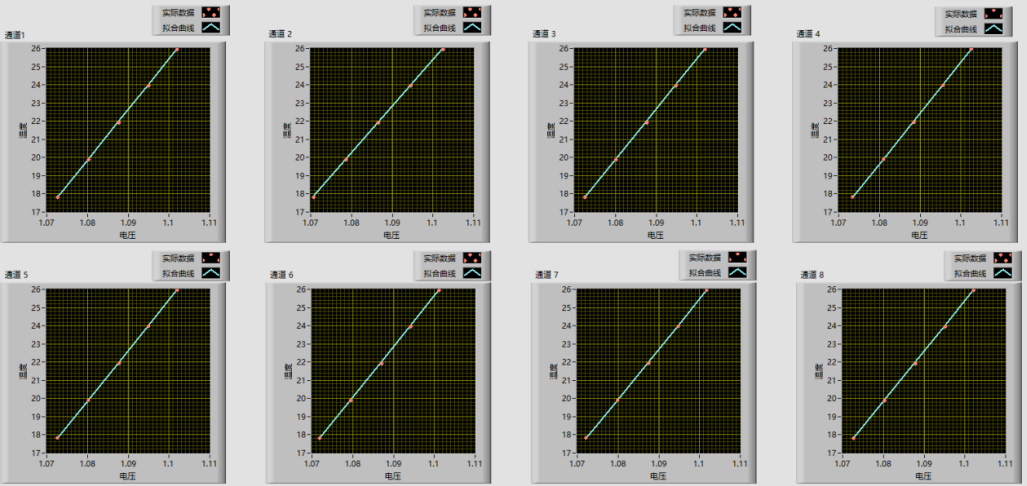
\includegraphics[width=12cm]{fig/3-fig/标定程序前面板.jpg}
    \caption{标定程序用户界面}
    \label{fig:标定程序用户界面}
\end{figure}